\documentclass[11pt, openany]{article}
%\usepackage{pstricks,pstricks-add,pst-math,pst-xkey}
\usepackage[frenchb]{babel}
%\usepackage{slashbox}
\usepackage{graphicx}
\usepackage{amsmath,amssymb,amstext}
\usepackage[latin1]{inputenc}
\usepackage[OT1]{fontenc}
%\usepackage{fancybox}
\usepackage{a4wide}
%\usepackage{fancyvrb}
\usepackage{pgf,tikz} %arbres
%\usetikzlibrary{arrows}
\usepackage{xcolor}
%\usepackage{multicol}
%\usepackage[cm]{fullpage}
\usepackage{amsthm} %pour les th�or�mes sans num�ro
\usepackage{array,multirow,makecell}
\usepackage{mathrsfs}

\usepackage{floatflt}

\usepackage{bussproofs}\EnableBpAbbreviations


\bibliographystyle{ieeetr}  


\newcounter{moncompteur}
\newtheorem{q}[moncompteur]{\textbf{Question}}{}
\newtheorem{prop}[moncompteur]{\textbf{Proposition}}{}
\newtheorem{df}[moncompteur]{\textbf{D�finition}}{}
\newtheorem*{df*}{\textbf{D�finition}}{}
\newtheorem{rem}[moncompteur]{\textbf{Remarque}}{}
\newtheorem{theo}[moncompteur]{\textbf{Th�or�me}}{}
\newtheorem*{theo*}{\textbf{Th�or�me}}{}
\newtheorem{conj}[moncompteur]{\textbf{Conjecture}}{}
\newtheorem{cor}[moncompteur]{\textbf{Corollaire}}{}
\newtheorem{lm}[moncompteur]{\textbf{Lemme}}{}
\newtheorem*{lm*}{\textbf{Lemme}}{}
%\newtheorem{nota}[moncompteur]{ \textbf{Notation}}{}
%\newtheorem{conv}[moncompteur]{ \textbf{Convention}}{}
\newtheorem{exa}[moncompteur]{\textbf{Exemple}}{}
\newtheorem{ex}[moncompteur]{\textbf{Exercice}}{}
%\newtheorem{app}[moncompteur]{ \textbf{Application}}{}
%\newtheorem{prog}[moncompteur]{ \textbf{Algorithme}}{}
%\newtheorem{hyp}[moncompteur]{ \textbf{Hypoth�se}}{}
%\newenvironment{dem}{\noindent\textbf{Preuve}\\}{\flushright$\blacksquare$\\}
%\newenvironment{dem}{\noindent\textbf{Preuve.} }{\hfill$\blacksquare$\\}

%\newenvironment{myindentpar}[1]%
%{\begin{list}{}%
%         {\setlength{\leftmargin}{#1}}%
%         \item[]%
%}
%{\end{list}}



%\newcommand{\R}{\mathbb{R}}
%\newcommand{\K}{\mathbb{K}}
%\newcommand{\N}{\mathbb{N}}
%\newcommand{\Z}{\mathbb{Z}}
%\newcommand{\C}{\mathbb{C}}
%\newcommand{\U}{\mathbb{U}}
%\newcommand{\Q}{\mathbb{Q}}
%\newcommand{\card}{\mathrm{card}}


\newcommand{\s}{\sigma}
%\newcommand{\l}{\lambda}
%\newcommand{\a}{\alpha}
%\newcommand{\r}{\rho}

%m�moire
\newcommand{\Ccal}{\mathcal{C}}
\newcommand{\Dcal}{\mathcal{D}}
\newcommand{\1}{\boldsymbol{1}}
\newcommand{\CProofs}{
%?\mathcal{C}?
\mathcal{CP}
}
%

\newcommand{\subsectionDescription}[1]{
\addtocontents{toc}{%\textit{
%\qquad\qquad
\hangindent=3.5\parindent \hangafter=0
\noindent
#1
}%}
}


\newcommand{\idees}[1]{
\textsf{(#1)}
}



%stage
\newcommand{\LK}{$\mathbf{LK}$}
\newcommand{\LJ}{$\mathbf{LJ}$}
\newcommand{\LJT}{$\mathbf{LJT}$}
\newcommand{\LSJ}{$\mathbf{LSJ}$}
\newcommand{\LSJn}{$\mathbf{LSJ\boldsymbol\ell}$}


\newcommand{\Sig}{\mathfrak S}
\newcommand{\G}{\Gamma}
\newcommand{\D}{\Delta}
\newcommand{\Th}{\Theta}
\newcommand{\Gp}{\Gamma}
\newcommand{\Dp}{\Delta}
\newcommand{\Gt}{\widetilde\Gamma}
\newcommand{\Dt}{\widetilde\Delta}

\newcommand{\imp}{\to\negthickspace}

\newcommand{\surj}{
%\mathrm{surj}
\boldsymbol
\Phi
}
\newcommand{\To}{\Rightarrow}
\newcommand{\forget}{\mathsf{forget}}



\newcommand{\autour}[5]{
^{#2}_{#3}#1^{#4}_{#5}
}




\begin{document}
%\renewcommand{\labelitemi}{$\diamond$}
\renewcommand{\labelitemi}{$\bullet$}
\vspace{2cm}~~\\


%regles et instances
\def\regle{
\def\defaultHypSeparation{\hskip .05in}
	\AXC	{$prem_{1}$}
	\AXC	{...}
	\AXC	{$prem_{p}$}
	\RightLabel{$(\mathcal R)$}
	\TIC{$concl$}
	\DP
}
\def\instance{
\def\defaultHypSeparation{\hskip .05in}
	\AXC	{$\s_{1}$}
	\AXC	{...}
	\AXC	{$\s_{p}$}
	\RightLabel{$(\mathcal R)$}
	\TIC{$\s$}
	\DP
}
\def\instanceAx{
\centerAlignProof
	\AXC	{\qquad}
	\RightLabel{$(\mathcal A)$}
	\UIC{$\s$}
	\DP
}
\def\instancedeux{
\def\defaultHypSeparation{\hskip .05in}
	\AXC	{$\s_{1}$}
	\AXC	{$\s_{2}$}
	\BIC{$\s$}
	\DP
}


%LJ
%LJ, axiomes
\def\LJid{
	\AXC	{}
	\RightLabel{$(id)$}
	\UIC{$A,\G \To A$}
	\DP
}
\def\LJbotL{
	\AXC	{}
	\RightLabel{$(\bot L)$}
	\UIC{$\bot,\G \To D$}
	\DP
}
%LJ,r�gles logiques
\def\LJetL{
	\AXC	{$A,B,\G \To D$}
	\RightLabel{$(\land L)$}
	\UIC{$A\land B,\G \To D$}
	\DP
}
\def\LJetR{
	\AXC	{$\G \To A$}
	\AXC	{$\G \To B$}
	\RightLabel{$(\land R)$}
	\BIC{$\G \To A\land B$}
	\DP
}
\def\LJouL{
	\AXC	{$A,\G \To D$}
	\AXC	{$B,\G \To D$}
	\RightLabel{$(\lor L)$}
	\BIC{$A\lor B,\G \To D$}
	\DP
}
\def\LJouRun{
	\AXC	{$\G \To A$}
	\RightLabel{$(\lor R_{1})$}
	\UIC{$\G \To A\lor B$}
	\DP
}
\def\LJouRdeux{
	\AXC	{$\G \To B$}
	\RightLabel{$(\lor R_{2})$}
	\UIC{$\G \To A\lor B$}
	\DP
}
\def\LJimpL{
	\AXC	{$\G \To A$}
	\AXC	{$B,\G \To D$}
	\RightLabel{$(\to L)$}
	\BIC{$A\to B,\G \To D$}
	\DP
}
\def\LJimpR{
	\AXC	{$A,\G \To B$}
	\RightLabel{$(\to R)$}
	\UIC{$\G \To A\to B$}
	\DP
}
%LJ, r�gles structurelles
\def\LJechange{
	\AXC	{$\G_{1},A,B,\G_{2} \To D$}
	\RightLabel{$(permut.\ L)$}
	\UIC{$\G_{1},B,A,\G_{2} \To D$}
	\DP
}
\def\LJcontraction{
	\AXC	{$A,A,\G \To D$}
	\RightLabel{$(contraction\ L)$}
	\UIC{$A,\G \To D$}
	\DP
}
\def\LJweakening{
	\AXC	{$\G \To D$}
	\RightLabel{$(weakening\ L)$}
	\UIC{$A,\G \To D$}
	\DP
}
%LJ, coupure
\def\LJcut{
	\AXC	{$\G_{1} \To A$}
	\AXC	{$A,\G_{2} \To D$}
	\RightLabel{$(cut)$}
	\BIC{$\G_{1},\G_{2} \To D$}
	\DP
}


%LK
\def\LKetR{
	\AXC	{$\G \To A,\D$}
	\AXC	{$\G \To B,\D$}
	\RightLabel{$(\land R)$}
	\BIC{$\G \To A\land B,\D$}
	\DP
}
\def\LKouR{
	\AXC	{$\G \To A,B,\D$}
	\RightLabel{$(\lor R)$}
	\UIC{$\G \To A\lor B,\D$}
	\DP
}

\def\LKTiersExclu{
	\AXC	{}
	\RightLabel{(id)}
	\UIC	{$A \To A, \bot$}
	\RightLabel{$(\to R)$}
	\UIC	{$\To A, (A\to\bot)$}
	\RightLabel{$(\lor R)$}
	\UIC{$\To A\lor (A\to\bot)$}
	\DP
}


%LJ ajustement
\def\LJimpLcontr{
	\AXC	{$\G,A\to B \To A$}
	\AXC	{$\G,B \To D$}
	\RightLabel{$(\to L)$}
	\BIC{$\G,A\to B \To D$}
	\DP
}
\def\LJimpLcontrA{
	\AXC	{$\G,A\to B \To A$}
	\AXC	{$\G,B \To A$}
	\RightLabel{$(\to L)$}
	\BIC{$\G,A\to B \To A$}
	\DP
}

\def\LJnnTiersExclu{
%	\AXC	{}
%	\RightLabel{id}
%	\UIC	{$A \To A, \bot$}
%	\RightLabel{$\to R$}
%	\UIC	{$\To A, (A\to\bot)$}
%	\RightLabel{$\lor R$}
	
	\AXC	{}
	\RightLabel{(id)}
	\UIC	{$A \;\To\; A$}
	\RightLabel{$(\lor R_{1})$}
	\UIC	{$A \;\To\; A\lor (A\to\bot)$}
	
		\AXC	{}
		\RightLabel{$(\bot L)$}
		\UIC	{$\bot,A \;\To\; \bot$}
	
	\RightLabel{$(\to L)$}
	\BIC	{$A,(A\lor (A\to\bot))\to\bot \;\To\; \bot$}
	\RightLabel{$(\to R)$}
	\UIC	{$(A\lor (A\to\bot))\to\bot \;\To\; A\to\bot$}
	\RightLabel{$(\lor R_{2})$}
	\UIC	{\colorbox{yellow}{$(A\lor (A\to\bot))\to\bot \;\To\; A\lor (A\to\bot)$}}
	
		\AXC	{}
		\RightLabel{$(\bot L)$}
		\UIC	{$\bot,(A\lor (A\to\bot))\to\bot \;\To\; \bot$}
	
	\RightLabel{$(\to L)$}
	\BIC	{$(A\lor (A\to\bot))\to\bot \,,\; (A\lor (A\to\bot))\to\bot \;\To\; \bot$}
	\RightLabel{$(contraction\ L)$}
	\UIC	{$(A\lor (A\to\bot))\to\bot \;\To\; \bot$}
	\RightLabel{$(\to R)$}
	\UIC{$\;\To\; ((A\lor (A\to\bot))\to\bot)\to\bot$}
	\DP
}





%LJT
\def\LJTimpLun{
	\AXC	{$B,A,\G \;\To\; D$}
	\RightLabel{$(\to L_{1})$}
	\UIC{$A\to B, A,\G \;\To\; D$}
	\DP
}
\def\LJTimpLdeux{
	\AXC	{$A_{1}\to(A_{2}\to B) \,,\; \G \;\To\; D$}
	\RightLabel{$(\to L_{2})$}
	\UIC{$(A_{1}\land A_{2})\to B \,,\; \G \;\To\; D$}
	\DP
}

%%%%%%%%%%%%

%LSJ

\def\LSJfauxL{
	\AXC	{}
	\RightLabel{$(\bot L)$}
	\UIC{$\Th\,; \bot, \G \To \D$}
	\DP
}
\def\LSJid{
	\AXC	{}
	\RightLabel{$(id)$}
	\UIC{$\Th\,; A,\G \To A,\D$}
	\DP
}
\def\LSJetL{
	\AXC{$\Th\,; A, B,\G \To \D$}
	\RightLabel{$(\land L)$}
	\UIC{$\Th\,; A\land B,\G \To  \D$}
	\DP
}
\def\LSJetR{
	\AXC{$\Th\,; \G \To A,\D$}
	\AXC{$\Th\,; \G \To B,\D$}
	\RightLabel{$(\land R)$}
	\BIC{$\Th\,; \G \To A\land B,\D$}
	\DP
}
\def\LSJouL{
	\AXC{$\Th\,; A,\G \To \D$}
	\AXC{$\Th\,; B,\G \To \D$}
	\RightLabel{$(\lor L)$}
	\BIC{$\Th\,; A\lor B,\G \To \D$}
	\DP
}
\def\LSJouR{
	\AXC{$\Th\,; \G \To A,B,\D$}
	\RightLabel{$(\lor R)$}
	\UIC{$\Th\,; \G \To A\lor B,\D$}
	\DP
}
\def\LSJimpL{
	\AXC{$\Th\,; B,\G \To \D$}
	\AXC{$B,\Th\,; \G \To A,\D$}
	\AXC{$B\,; \Th,\G \To A$}
	\RightLabel{$(\to L)$}
	\TIC{$\Th\,; A\to B,\G \To \D$}
	\DP
}
\def\LSJimpR{
	\AXC{$\Th\,; A,\G \To B,\D$}
	\AXC{$\emptyset\,; A,\Th,\G \To B$}
	\RightLabel{$(\to R)$}
	\BIC{$\Th\,; \G \To A\to B,\D$}
	\DP
}



% LSJL


\def\LSJLfauxL{
	\AXC	{}
	\RightLabel{$(\bot L)$}
	\UIC{$i:\bot, \Gp \To_{n} \Dp$}
	\DP
}
\def\LSJLid{
	\AXC	{}
	\RightLabel{$(id)$}
	\UIC{$i:A,\Gp \To_{n} n:A,\Dp$}
	\DP
}
\def\LSJLetL{
	\AXC{$i:A,i:B,\Gp \To_{n} \Dp$}
	\RightLabel{$(\land L)$}
	\UIC{$i:A\land B,\Gp \To_{n} \Dp$}
	\DP
}
\def\LSJLetR{
	\AXC{$\Gp \To_{n} n:A,\Dp$}
	\AXC{$\Gp \To_{n} n:B,\Dp$}
	\RightLabel{$(\land R)$}
	\BIC{$\Gp \To_{n} n:A\land B,\Dp$}
	\DP
}
\def\LSJLouL{
	\AXC{$i:A,\Gp \To_{n} \Dp$}
	\AXC{$i:B,\Gp \To_{n} \Dp$}
	\RightLabel{$(\lor L)$}
	\BIC{$i:A\lor B,\Gp \To_{n} \Dp$}
	\DP
}
\def\LSJLouR{
	\AXC{$\Gp \To_{n} n:A,n:B,\Dp$}
	\RightLabel{$(\lor R)$}
	\UIC{$\Gp \To_{n} n:A\lor B,\Dp$}
	\DP
}
\def\LSJLimpL{
	\AXC{$i:B,\Gp \To_{n} \Dp$}
	\AXC{$n+1:B,\Gp \To_{n} n:A,\Dp$}
	\AXC{$n+2:B,\Gp \To_{n+1} n+1:A, \Dp$}
	\RightLabel{$(\to L)$}
	\TIC{$i:A\to B,\Gp \To_{n} \Dp$}
	\DP
}
\def\LSJLimpR{
	\AXC{$0:A,\Gp \To_{n} n:B,\Dp$}
	\AXC{$0:A,\Gp \To_{n+1} n+1:B, \Dp$}
	\RightLabel{$(\to R)$}
	\BIC{$\Gp \To_{n} n:A\to B,\Dp$}
	\DP
}


% �quivalence LSJL LSJ

\def\instanceR{
\def\defaultHypSeparation{\hskip .05in}
	\AXC	{$\s_{1}$}
	\AXC	{...}
	\AXC	{$\s_{p}$}
	\RightLabel{$(\mathcal R)$}
	\TIC{$\s$}
	\DP
}
\def\instanceRp{
\def\defaultHypSeparation{\hskip .05in}
	\AXC	{$\s'_{1}$}
	\AXC	{...}
	\AXC	{$\s'_{p}$}
	\RightLabel{$(\mathcal R')$}
	\TIC{$\s'$}
	\DP
}
\def\instanceAx{
\centerAlignProof
	\AXC	{\qquad}
	\RightLabel{$(\mathcal A)$}
	\UIC{$\s$}
	\DP
}
\def\instanceAxp{
\centerAlignProof
	\AXC	{\qquad}
	\RightLabel{$(\mathcal A')$}
	\UIC{$\s'$}
	\DP
}
\def\instanceid{
\centerAlignProof
	\AXC	{\qquad}
	\RightLabel{(id)}
	\UIC{$\s$}
	\DP
}
\def\instanceidp{
\centerAlignProof
	\AXC	{\qquad}
	\RightLabel{(id$'$)}
	\UIC{$\s'$}
	\DP
}
\def\instanceetR{
\def\defaultHypSeparation{\hskip .05in}
	\AXC	{$\s_{1}$}
	\AXC	{$\s_{2}$}
	\RightLabel{$(\land R)$}
	\BIC{$\s$}
	\DP
}
\def\instanceetRp{
\def\defaultHypSeparation{\hskip .05in}
	\AXC	{$\s'_{1}$}
	\AXC	{$\s'_{2}$}
	\RightLabel{($\land R'$)}
	\BIC{$\s'$}
	\DP
}
\def\instanceimpL{
\def\defaultHypSeparation{\hskip .in}
	\AXC	{$\s_{1}$}
	\AXC	{$\s_{2}$}
	\AXC	{$\s_{3}$}
	\RightLabel{($\to L$)}
	\TIC{$\s$}
	\DP
}
\def\instanceimpLp{
\def\defaultHypSeparation{\hskip .in}
	\AXC	{$\s'_{1}$}
	\AXC	{$\s'_{2}$}
	\AXC	{$\s'_{3}$}
	\RightLabel{($\to L'$)}
	\TIC{$\s'$}
	\DP
}





\tableofcontents

\pagebreak





% def cat�gorie
\begin{df}
Une \textbf{\emph{cat�gorie}} consiste en une collection d'\emph{objets} et une collection de \emph{morphismes}, cette derni�re munie d'une op�rations binaire partielle $\circ$ appel�e \emph{composition}, avec les propri�t�s suivantes.

\begin{itemize}

\item
\`A chaque morphisme $f$ est associ� un couple d'objets $(A,B)$ ; on �crit $f:A\to B$.
On dit que $A\to B$ est le \emph{type} de $f$, et que $f$ est un morphisme \emph{de} $A$ \emph{vers} $B$, et encore que $A$ est le \emph{domaine} ou la \emph{source} de $f$, et $B$ le \emph{codomaine} ou la \emph{cible} de $f$.

\item
Pour tous objets $A$, $B$, $C$ et morphismes $f$, $g$ tels que $f:A\to B$ et $g:B\to C$, le morphisme $g\circ f$ existe et $g\circ f:A\to C$.

\item
\textbf{Identit�.}
Pour tout objet $A$, il existe un morphisme particulier $id_{A}:A\to A$ appel� \emph{identiti� sur $A$}, tel que 
%pour tous objet $B$ et morphismes $f:B\to A$ et $g:A\to B$, $id_{A}\circ f=f$ et $g\circ id_{A}=g$.
pour tout objet $B$, pour tout $f:B\to A$, $id_{A}\circ f=f$ et pour tout $g:A\to B$, $g\circ id_{A}=g$.

\item
\textbf{Associativit�.}
Pour tous $f:A\to B$, $g:B\to C$, $h:C\to D$, on a $h\circ(g\circ f) = (h\circ g)\circ f$.

\end{itemize}
\end{df}

On d�signe souvent une cat�gorie par la collection de ses objets.


% def cat�gorie mono�dale
\begin{df}
%Une \textbf{\emph{cat�gorie mono�dale}} est une cat�gorie $\C$ munie d'un bifoncteur ${\otimes:\C\times\C \longrightarrow \C}$ tel que
%
%\begin{itemize}
%%\item
%%pour tous objets $A$, $B$, $C$, il existe une isomorphisme naturel d'associativit�
%%\linebreak
%%${\alpha_{A,B,C} : (A\otimes B)\otimes C \to A\otimes(B\otimes C)}$ ;
%%\item
%%il existe un objet $e$, unitaire
%\item
%une \textbf{associativit�} est fournie par un morphisme naturel pour tous objets $A$, $B$, $C$ : ${\alpha_{A,B,C} : (A\otimes B)\otimes C \to A\otimes(B\otimes C)}$ ;
%\item
%il existe un objet $e$ \textbf{unitaire} gr�ce � des morphismes naturels pour tout objet $A$ : ${\lambda_{A}:e\otimes A\to A}$ et ${\rho_{A}:A\otimes e\to A}$.
% 
%\end{itemize}

Une \textbf{\emph{cat�gorie mono�dale}} est une cat�gorie $\C$ munie d'un bifoncteur ${\otimes:\C\times\C \longrightarrow \C}$ et d'un objet $e$, tel que les morphismes suivants existent

\begin{itemize}
\item
pour tous objets $A$, $B$, $C$, un isomorphisme
%\linebreak
${\alpha_{A,B,C} : (A\otimes B)\otimes C \to A\otimes(B\otimes C)}$ permettant de parler d'associativit� ;
\item
pour tout objet $A$, des isomorphismes ${\lambda_{A}:e\otimes A\to A}$ et ${\rho_{A}:A\otimes e\to A}$ justifiant le nom d'\textbf{unit�} pour $e$ ;
\end{itemize}

\noindent
et tel que les diagrammes suivants commutent pour tous objets $A$, $B$, $C$, $D$. On a omis les indices de $\alpha$, $\lambda$, $\rho$ et �crit $A$ pour $id_{A}$ : par exemple, comprendre $\alpha\otimes D$ comme $\alpha_{A,B,C}\otimes id_{A}$.

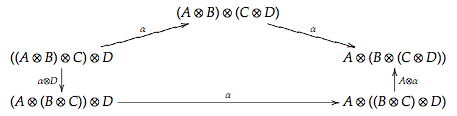
\includegraphics[width=\linewidth]{diagrammeMonoidalePenta}
\centering{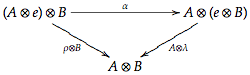
\includegraphics[width=0.5\linewidth]{diagrammeMonoidaleTri}}

\end{df}





\pagebreak

\`A chaque preuve $\pi$ on associe une \emph{d�notation} $[\pi]$, qu'on veut invariante par �limination de la coupure.

\

Les objets sont les formules et les morphismes sont des d�notations de preuves. Les morphismes d'une formule $A$ vers une formule $B$ sont les d�notations des diff�rentes preuves du s�quent $A\vdash B$ (si le s�quent n'est pas prouvable, il n'y en a pas).

Soit $A$, $B$, $C$ des formules, $\pi_{1}$ une preuve de $A\vdash B$ et $\pi_{2}$ une preuve de $B\vdash C$. On d�finit $[\pi_{2}]\circ[\pi_{1}]$ comme la d�notation de la preuve suivante de $A\vdash C$
\begin{prooftree}
	\AXC	{$\pi_{1}$}
	\noLine
	\UIC{$A\vdash B$}
	\AXC	{$\pi_{2}$}
	\noLine
	\UIC{$B\vdash C$}
	\RightLabel{$(cut)$}
	\BIC{$A\vdash C$}
\end{prooftree}

L'identit� $id_{A}$ sur une formule $A$ est la d�notation de la preuve
{\centerAlignProof
	\AXC	{}
	\RightLabel{$(Id)$}
	\UIC{$A\vdash A$}
	\DP
}.
Soit $\pi$ une preuve de $A\vdash B$, l'�limination de la coupure transforme la preuve
\\
\begin{center}
	\AXC	{}
	\RightLabel{$(Id)$}
	\UIC{$A\vdash A$}
	\AXC	{$\pi$}
	\noLine
	\UIC{$A\vdash B$}
	\RightLabel{$(cut)$}
	\BIC{$A\vdash B$}
	\DP
\qquad\qquad en \qquad\qquad
	\AXC	{$\pi$}
	\noLine
	\UIC{$A\vdash B$}
	\DP
\end{center}

\noindent
donc on a bien $[\pi]\circ id_{A}=[\pi]$. De m�me pour $\pi$ une preuve de $B\vdash A$, on a $id_{A}\circ[\pi]=[\pi]$.

L'associativit� vient de ce que les preuves
\\
\begin{center}
	\AXC	{$\pi_{1}$}
	\noLine
	\UIC{$A\vdash B$}
	\AXC	{$\pi_{2}$}
	\noLine
	\UIC{$B\vdash C$}
	\RightLabel{$(cut)$}
	\BIC{$A\vdash C$}
	\AXC	{$\pi_{3}$}
	\noLine
	\UIC{$C\vdash D$}
	\RightLabel{$(cut)$}
	\BIC{$A\vdash D$}
	\DP
\quad et \quad
	\AXC	{$\pi_{1}$}
	\noLine
	\UIC{$A\vdash B$}
	\AXC	{$\pi_{2}$}
	\noLine
	\UIC{$B\vdash C$}
	\AXC	{$\pi_{3}$}
	\noLine
	\UIC{$C\vdash D$}
	\RightLabel{$(cut)$}
	\BIC{$B\vdash D$}
	\RightLabel{$(cut)$}
	\BIC{$A\vdash D$}
	\DP
\end{center}

\noindent
sont �quivalentes � �limination de la coupure pr�s.







\end{document}
